\documentclass[11pt]{article}
\usepackage[margin=0.9in]{geometry}
\usepackage{amsmath,amssymb,graphicx,booktabs,hyperref,xcolor,float}
\usepackage[T1]{fontenc}\usepackage{lmodern}
\usepackage{listings}
\lstset{basicstyle=\ttfamily\scriptsize,breaklines=true,columns=fullflexible,frame=single,language=Python,showstringspaces=false}
\graphicspath{{../v3/}}
\newcommand{\hmpc}{\,h\,\mathrm{Mpc}^{-1}}
\newcommand{\kmax}{k_{\max}}
\title{FLAMINGO versus the NLA and TATT best fits, and the goodness of fit as $\chi^2/\nu$\\[2pt]\large Companion to the scale-cut summary (production truth)}
\author{Yijie Zhu, with Claude}
\date{9 November 2026}

\begin{document}
\maketitle

\section*{Summary}

Two things, both on the production truth of the main summary (measured
FLAMINGO spectra, $N_s$ fixed to the B-mode plateau, three probes $P_{hE}$,
$P_{EE}$, $P_{BB}$, $k \ge 0.05\hmpc$):
\begin{enumerate}
\item \textbf{Direct comparison of the spectra with the best fits}
  (Section~2). For six snapshots ($z$ = 0.2, 0.5, 0.75, 1, 1.5, 2) and three
  fit ranges ($k \le 0.16$, 0.29, 0.52$\hmpc$) the GI and II ratios to
  $P_{\rm NL}$ are shown with the measured points, the smoothed truth and the
  NLA and TATT best fits, each with a panel of the residual model/measured $-1$ at the
  measured points with their error bars. The pictures make the two failure modes visible: NLA
  predicts a $k$-independent ratio for both GI and II, while the simulation's
  GI ratio dips by 7 to 26 per cent at $k \simeq 0.7$ to 1.3$\hmpc$
  (strongest at low $z$) and its II ratio rises steadily from $k \simeq 0.1$;
  TATT follows the II rise to $k \simeq 0.3$ to 0.5 and the GI shape to
  $k \simeq 0.3$, then bends the wrong way on GI (30 to 65 per cent above the
  truth at $k \simeq 1$ for $z \le 1$ when anchored at 0.16) and flattens on II. B modes:
  TATT predicts the right order of magnitude to $k \simeq 0.3$ and falls short
  beyond; NLA predicts none.
\item \textbf{Goodness of fit as $\chi^2/\nu$} (Section~3). The $p$-value
  of the main summary is rewritten as the reduced chi-square
  $\chi^2_{\min}(\kmax)/\nu$, $\nu = 3N_k(\kmax) - n_{\rm par}$, with the exact
  mapping $p = 0.05 \Leftrightarrow \chi^2/\nu = \chi^2_{0.95}(\nu)/\nu$,
  which runs from 2.2 (NLA, $\nu = 5$) down to 1.4 ($\nu = 40$). Tables of
  $\chi^2/\nu$ at every $\kmax$ and the cuts obtained with fixed thresholds
  1.5, 2 and 3 are given. A fixed threshold of 2 reproduces the $p$-rule cuts
  in 13 of 18 cases (the other five differ by one grid step); a threshold of
  3 moves the cuts one to two grid steps outward (NLA 0.09 to 0.16, TATT
  0.29 to 0.52). The
  core-combined $\chi^2/\nu$ is 2.1 / 2.7 / 4.8 / 9.2 (NLA) and 0.84 / 0.77 /
  1.0 / 1.5 (TATT) at $\kmax$ = 0.12 / 0.16 / 0.22 / 0.29$\hmpc$.
\end{enumerate}

\section{Set-up and definitions}

\paragraph{Data.} For each snapshot $s$ at redshift $z_s$ the measured
FLAMINGO spectra $y_{s,X}(k)$, $X \in \{hE, EE, BB\}$, with errors
$\sigma_{s,X}(k)$ on the 26 $k$ nodes (20 of them at $k \ge 0.05\hmpc$ up to
$3.04\hmpc$ in the fit range). The smoothed truth $T_{s,X}(k)$ is the
smoothing spline of the main summary; $N_s$ is the B-mode plateau, kept fixed
in every fit. Conversion to the cosmolike convention as always:
$P_{\delta E} = P_{hE}/b$, $b(k) = \sqrt{P_{hh}/P_{\rm NL}}$, so the GI ratio
plotted is
\begin{equation}
  R_{\rm GI}(k) = -\frac{P_{\delta E}}{P_{\rm NL}} = -\frac{P_{hE}}{b\,P_{\rm NL}},
  \qquad
  R_{\rm II}(k) = \frac{P_{EE} - N_s}{P_{\rm NL}},
  \qquad
  R_{\rm BB}(k) = \frac{P_{BB} - N_s}{P_{\rm NL}} .
\end{equation}
The lower panels show the residual at the measured points,
$100\,(M/y - 1)$ with $M$ the model and $y$ the measured spectrum, computed on
the same quantity (numerator only, $N_s$ subtracted for II and BB), with the
measured error bars $\pm 100\,\sigma/|y|$ (identical for the two models, the
points are offset by 1.5 per cent in $k$ so both are visible). The thin grey
line is the smoothed truth $T$ shown the same way, $100\,(T/y - 1)$, so the
distance between a model and the grey line is the model's deviation from the
truth, and the distance from zero is its deviation from the data. The
percentages quoted in Section~2 are model versus smoothed truth. Note that
the measured errors shrink from 4 to 6 per cent at $k \le 0.09$ to 1 per cent
at $k \simeq 0.3$ (GI), so the fit of a constant (NLA) is pinned by the
highest-$k$ points in range: a 3 to 10 per cent residual at $k < 0.1$ is
within one to two error bars and is where the fit is least constrained, not
where the model is worst.

\paragraph{Models.} NLA: $P_{\delta E} = -C_1 P_{\rm NL}$, $P_{EE} = C_1^2 P_{\rm NL}$,
$P_{BB} = 0$ with $C_1 = A_1\,\bar C_1 \rho_{\rm crit}\Omega_m/D(z)$; one free
parameter $A_1$. TATT: the full quadratic expansion (density weighting $b_{TA}$,
tidal torque $A_2$, $C_2 = A_2 \bar C_1 \rho_{\rm crit}\Omega_m / D^2$) with
the kernels of \texttt{fit\_tatt\_flamingo.TATTModel} evaluated on the FLAMINGO
$P_{\rm NL}$; three free parameters $(A_1, A_2, b_{TA})$, bounded to the chain
priors ($A_1 \in [0, 20]$, $A_2 \in [-5, 5]$, $b_{TA} \in [0, 2]$). The NLA
ratios $R_{\rm GI}$ and $R_{\rm II}$ are therefore constants in $k$ at every
redshift, which is the single most useful thing to keep in mind when reading
the figures.

\paragraph{Fit.} At each $\kmax$ on the grid of data nodes (0.09, 0.12, 0.16, 0.22, 0.29,
0.39, 0.52, 0.70, 0.94, 1.26, 1.69, 2.27, 3.04$\hmpc$) the parameters
minimise
\begin{equation}
  \chi^2(\kmax) = \sum_{X \in \{hE, EE, BB\}}\ \sum_{0.05 \le k_i \le \kmax}
  \left[\frac{y_{s,X}(k_i) - M_{s,X}(k_i)}{\sigma_{s,X}(k_i)}\right]^2 ,
\end{equation}
diagonal errors, $N_s$ added to the model $EE$ and $BB$. The best-fit
parameters shown here are the stored ones of the main summary
(\texttt{v3/v3.npz}); the model curves are recomputed from them with the same
prediction code, so the figures and the $\chi^2$ tables are the same fits.

\section{FLAMINGO versus the best fits}

Figures~\ref{fig:gi16} to \ref{fig:bb29} show the comparison for the fit
ranges $k \le 0.16$ (the anchor range of the main summary, where both models
pass), $k \le 0.29$ (the TATT GoF cut at most redshifts; NLA has failed by
then) and $k \le 0.52$ (both models fail; shows how the fits compromise when
pushed). Everything to the right of the dashed line (shaded) is an
extrapolation of that fit.

\paragraph{GI (Fig.~\ref{fig:gi16}, \ref{fig:gi29}, \ref{fig:gi52}).}
The simulation's $|R_{\rm GI}|$ is flat to $k \simeq 0.2$, dips to a minimum
at $k \simeq 0.7$ to 1.3 (relative to the $k = 0.1$ value: 0.74 at $z = 0.2$,
0.76 at 0.5, 0.83 at 0.75, 0.93 at 1; no dip at $z \ge 1.5$) and then rises
steeply (1.2 to 1.6 times the large-scale value by $k = 3$). NLA, being a
constant, is within 3 to 8 per cent of the truth inside the $k \le 0.16$
range at every redshift and misses the dip entirely (+10 to +38 per cent at
$k \simeq 0.7$ to 1.3 for $z \le 1$). TATT anchored at 0.16 is within 1 to 5
per cent in range, follows the start of the dip to $k \simeq 0.3$, and then
turns upward instead of downward: with $A_2 \simeq -0.9$ and $b_{TA} \simeq 0.3$
to 0.6 the quadratic terms grow as $P^2$-like kernels and overshoot the truth
by 30 to 65 per cent at $k \simeq 1$. Fitting to $k \le 0.29$ (the TATT cut)
moves $A_2$ to $-1.2$ to $-1.3$ and reduces $b_{TA}$; the in-range error stays
at or below 6 per cent for TATT (3.5 to 11 per cent for NLA, which is now failing on
II rather than GI). Fitting to $k \le 0.52$ forces TATT to compromise: 10 to
16 per cent in-range errors at $z \le 0.75$, with $b_{TA} \to 0$ at low $z$.
At $z = 2$ the snapshot behaves differently (the GI ratio rises
monotonically; $A_2$ flips sign to $+2$ in the 0.16 and 0.29 fits), the
anomaly already noted in the main summary.

\paragraph{II (Fig.~\ref{fig:ii16}, \ref{fig:ii29}, \ref{fig:ii52}).}
$R_{\rm II}$ rises from $k \simeq 0.1$ at every redshift, by a factor 1.5 to 3
between $k = 0.1$ and 1 and by 3 to 6 by $k = 3$: the signature of the
white (one-halo-like) E-mode excess of the main summary, which with $N_s$
fixed to the B plateau cannot be absorbed. Because $P_{hE}$ carries much
smaller fractional errors than $P_{EE}$, the fits are driven by GI and the II
residual is what fails first. NLA, a constant, under-predicts II by 13 to 19
per cent already inside $k \le 0.16$ and by 22 to 32 per cent inside
$k \le 0.29$ (the 0.16 fit is 26 to 55 per cent low at $k = 0.52$); this is
why the NLA cut sits at 0.09 to 0.12 although its GI residual alone would
allow 0.3. TATT tracks the II rise to within 2 to 10 per cent in range at
0.16 and 4 to 22 per cent at 0.29 (worst at $z = 0.2$), and is within
$\pm 15$ per cent at $k = 0.52$ for $z \ge 0.5$; beyond that its II flattens
while the simulation keeps rising. Pushed to $k \le 0.52$ the TATT II error in
range grows to 20 to 50 per cent at $z \le 1$ as the fit trades II against GI.

\paragraph{B modes (Fig.~\ref{fig:bb29}).} The B-mode excess above the
plateau rises like II. TATT (whose B mode comes from $b_{TA}^2$, $b_{TA}A_2$ and
$A_2^2$ terms) matches it in amplitude to $k \simeq 0.3$ and falls a factor
of several to ten short by $k = 3$; NLA predicts no B mode. The B-mode points carry
little weight in the $\chi^2$ (large errors), so they do not drive the cuts.

\begin{figure}[H]\centering
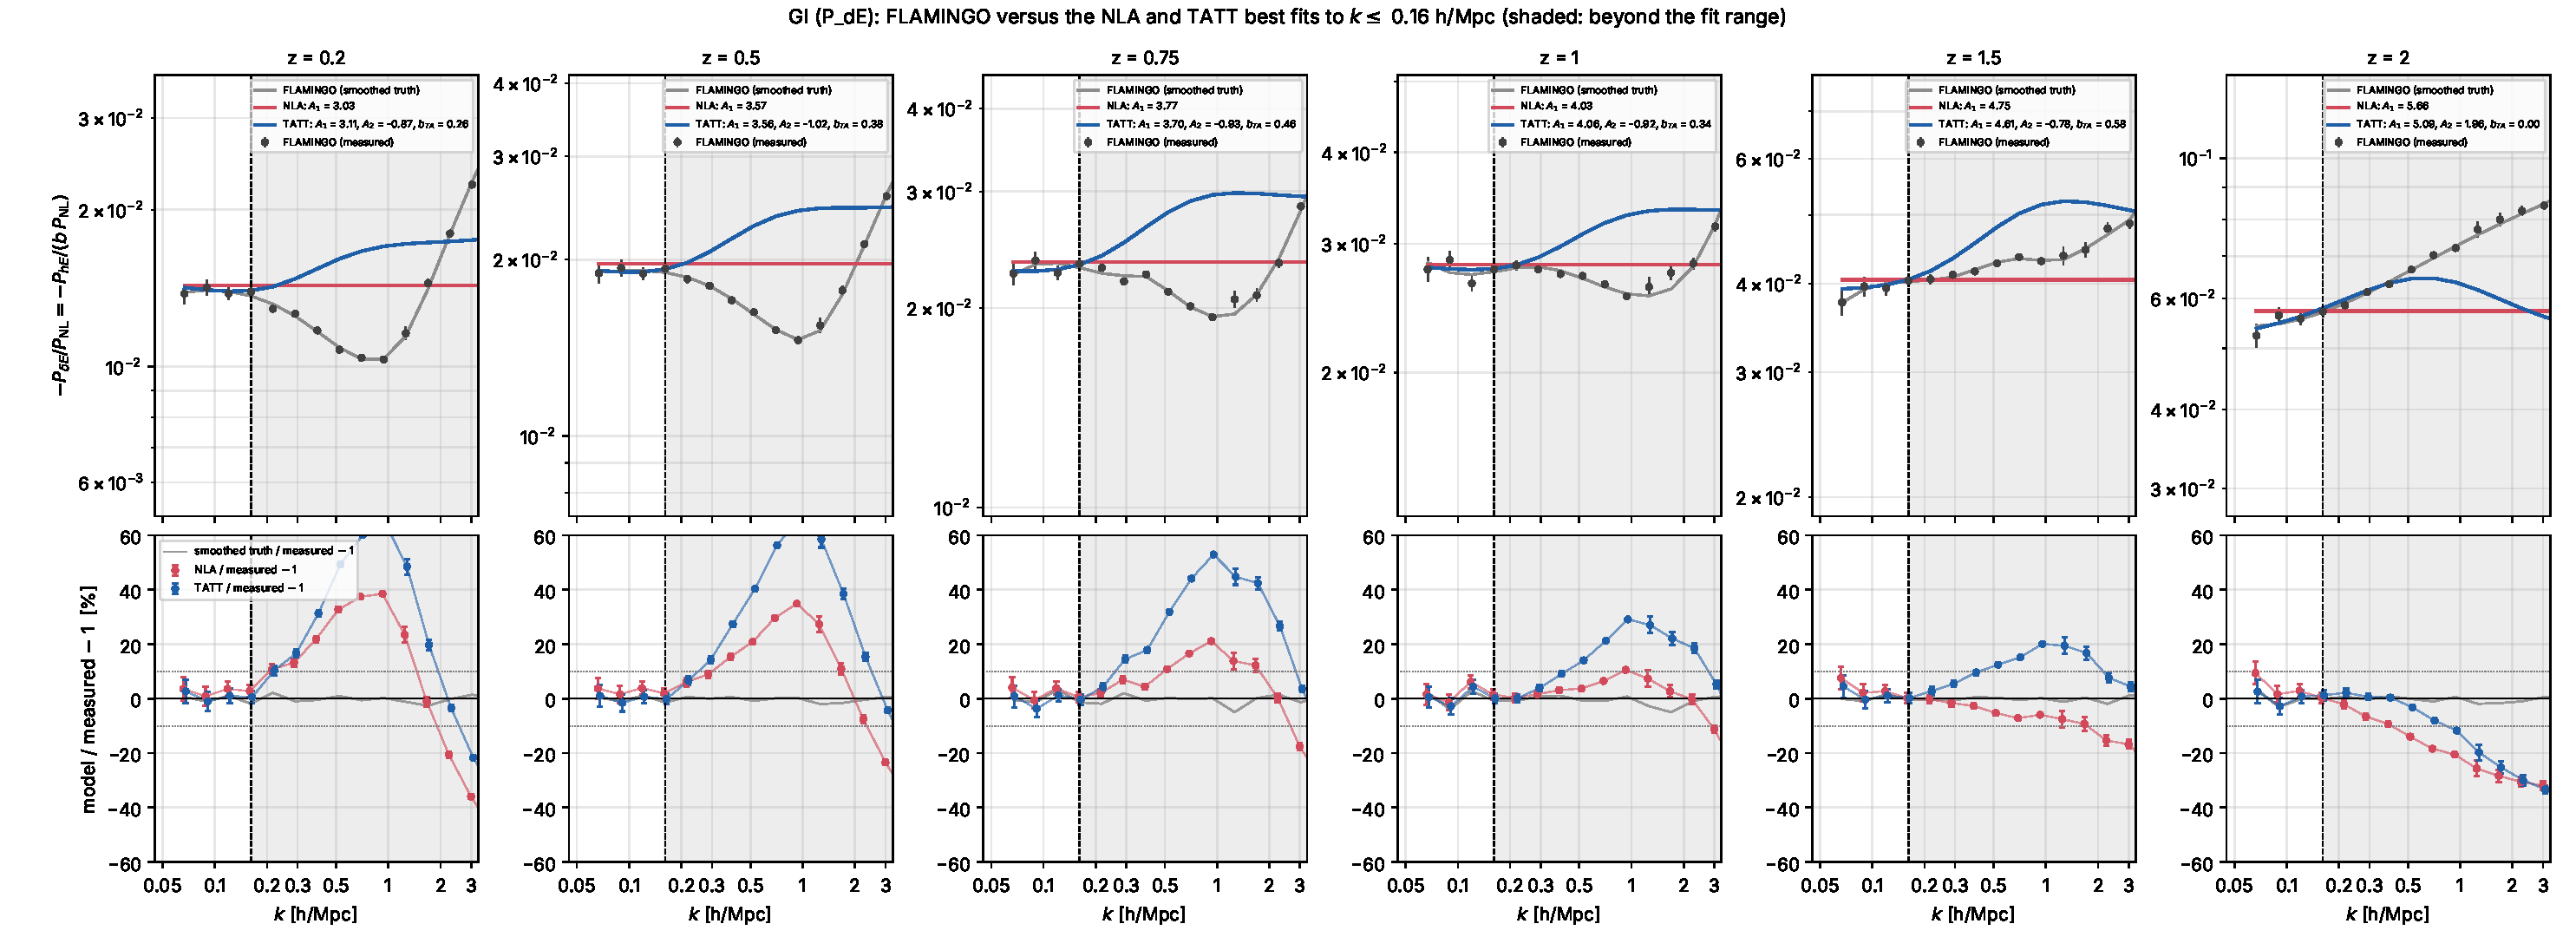
\includegraphics[width=\textwidth]{fig_cmp_GI_k0p16}
\caption{GI: FLAMINGO (points: measured with errors; grey line: smoothed
truth) against the NLA and TATT best fits to $k \le 0.16\hmpc$ (the anchor
range). Lower panels: model/measured $-1$ in per cent at every node with the
measured error bars; thin grey line the smoothed truth relative to the
measured points; dotted lines $\pm 10$ per cent. Shaded: beyond the fit
range.}
\label{fig:gi16}
\end{figure}
\begin{figure}[H]\centering
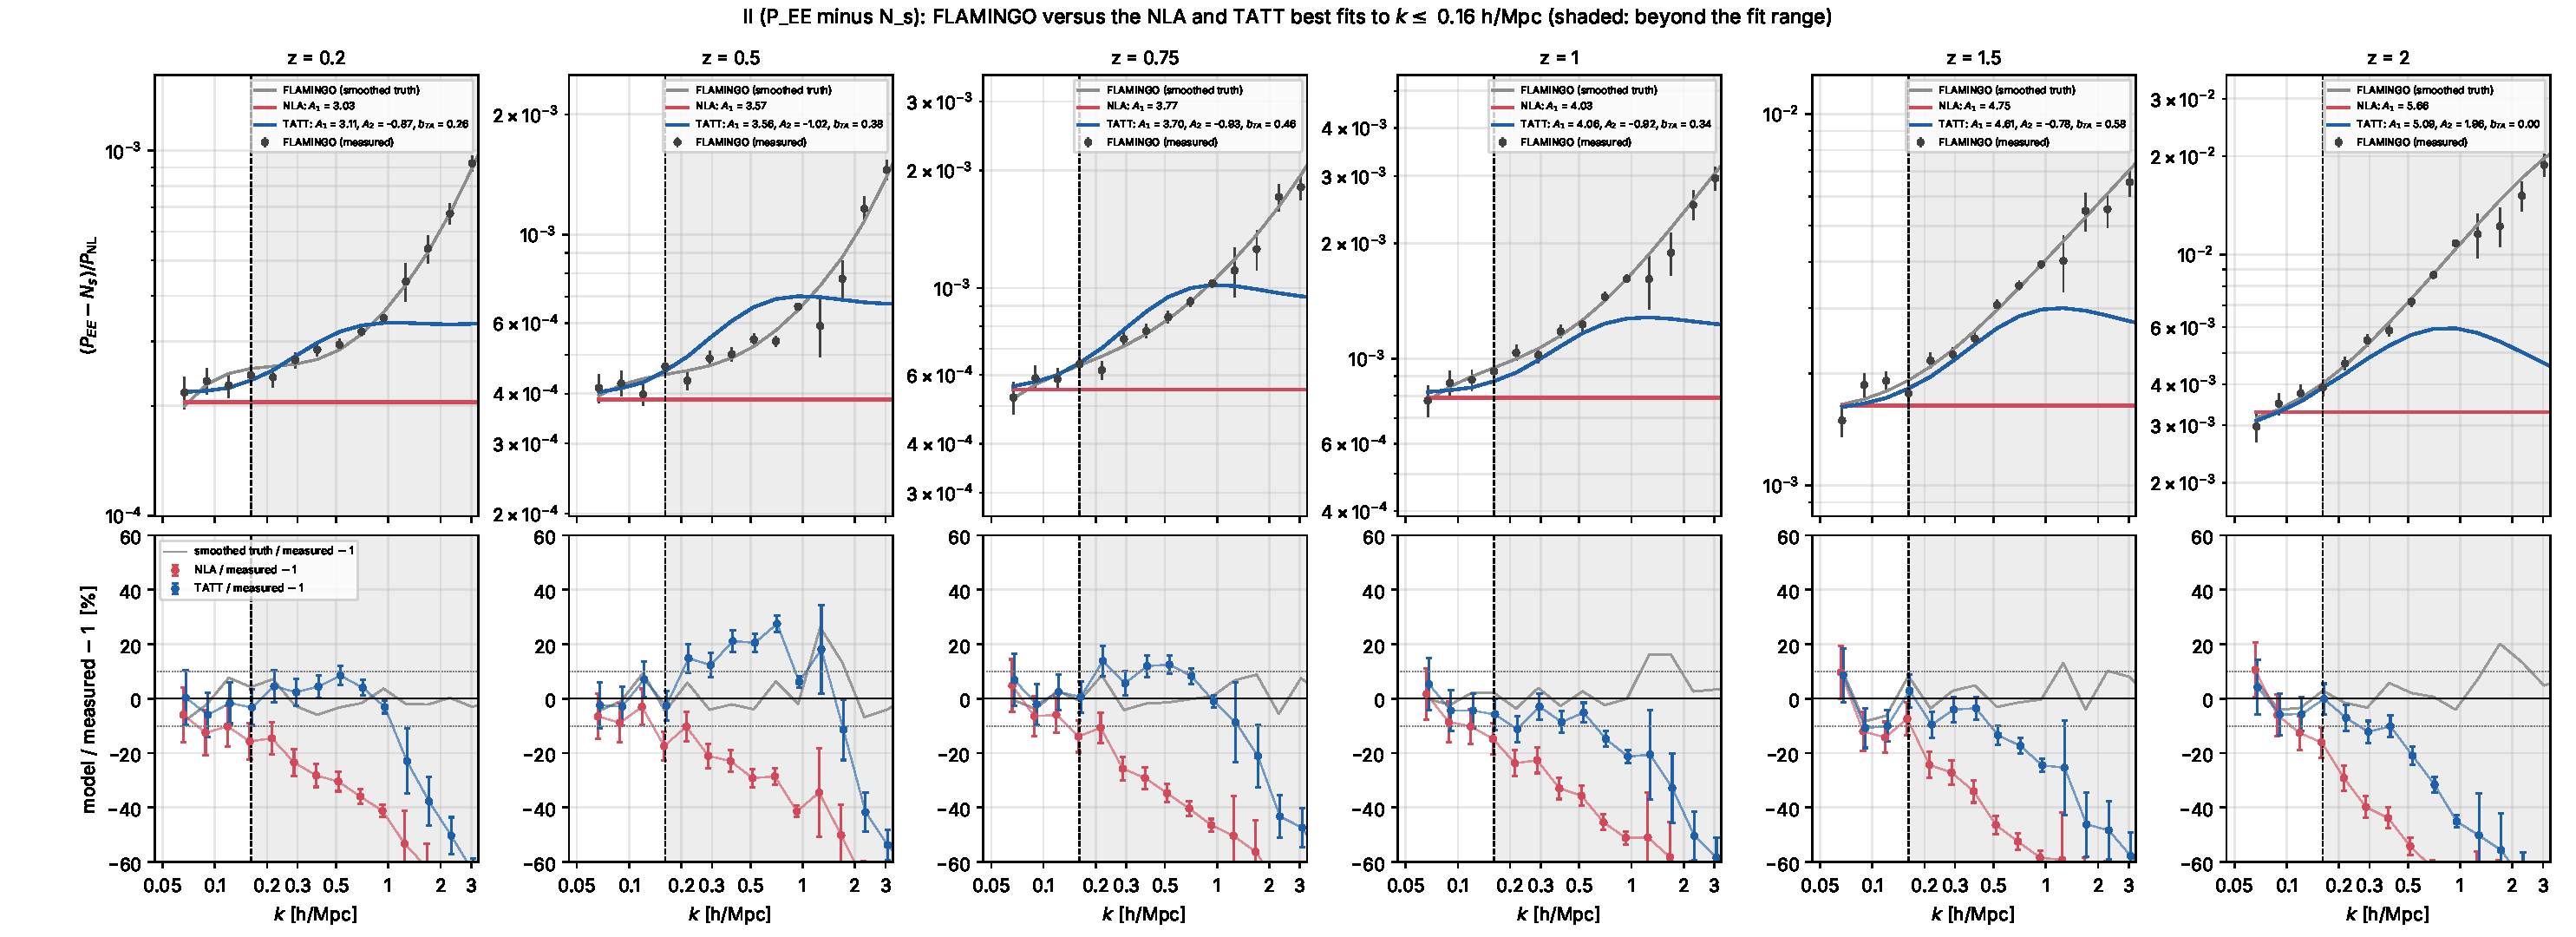
\includegraphics[width=\textwidth]{fig_cmp_II_k0p16}
\caption{II ($P_{EE} - N_s$), fits to $k \le 0.16\hmpc$. Same layout as
Fig.~\ref{fig:gi16}.}
\label{fig:ii16}
\end{figure}
\begin{figure}[H]\centering
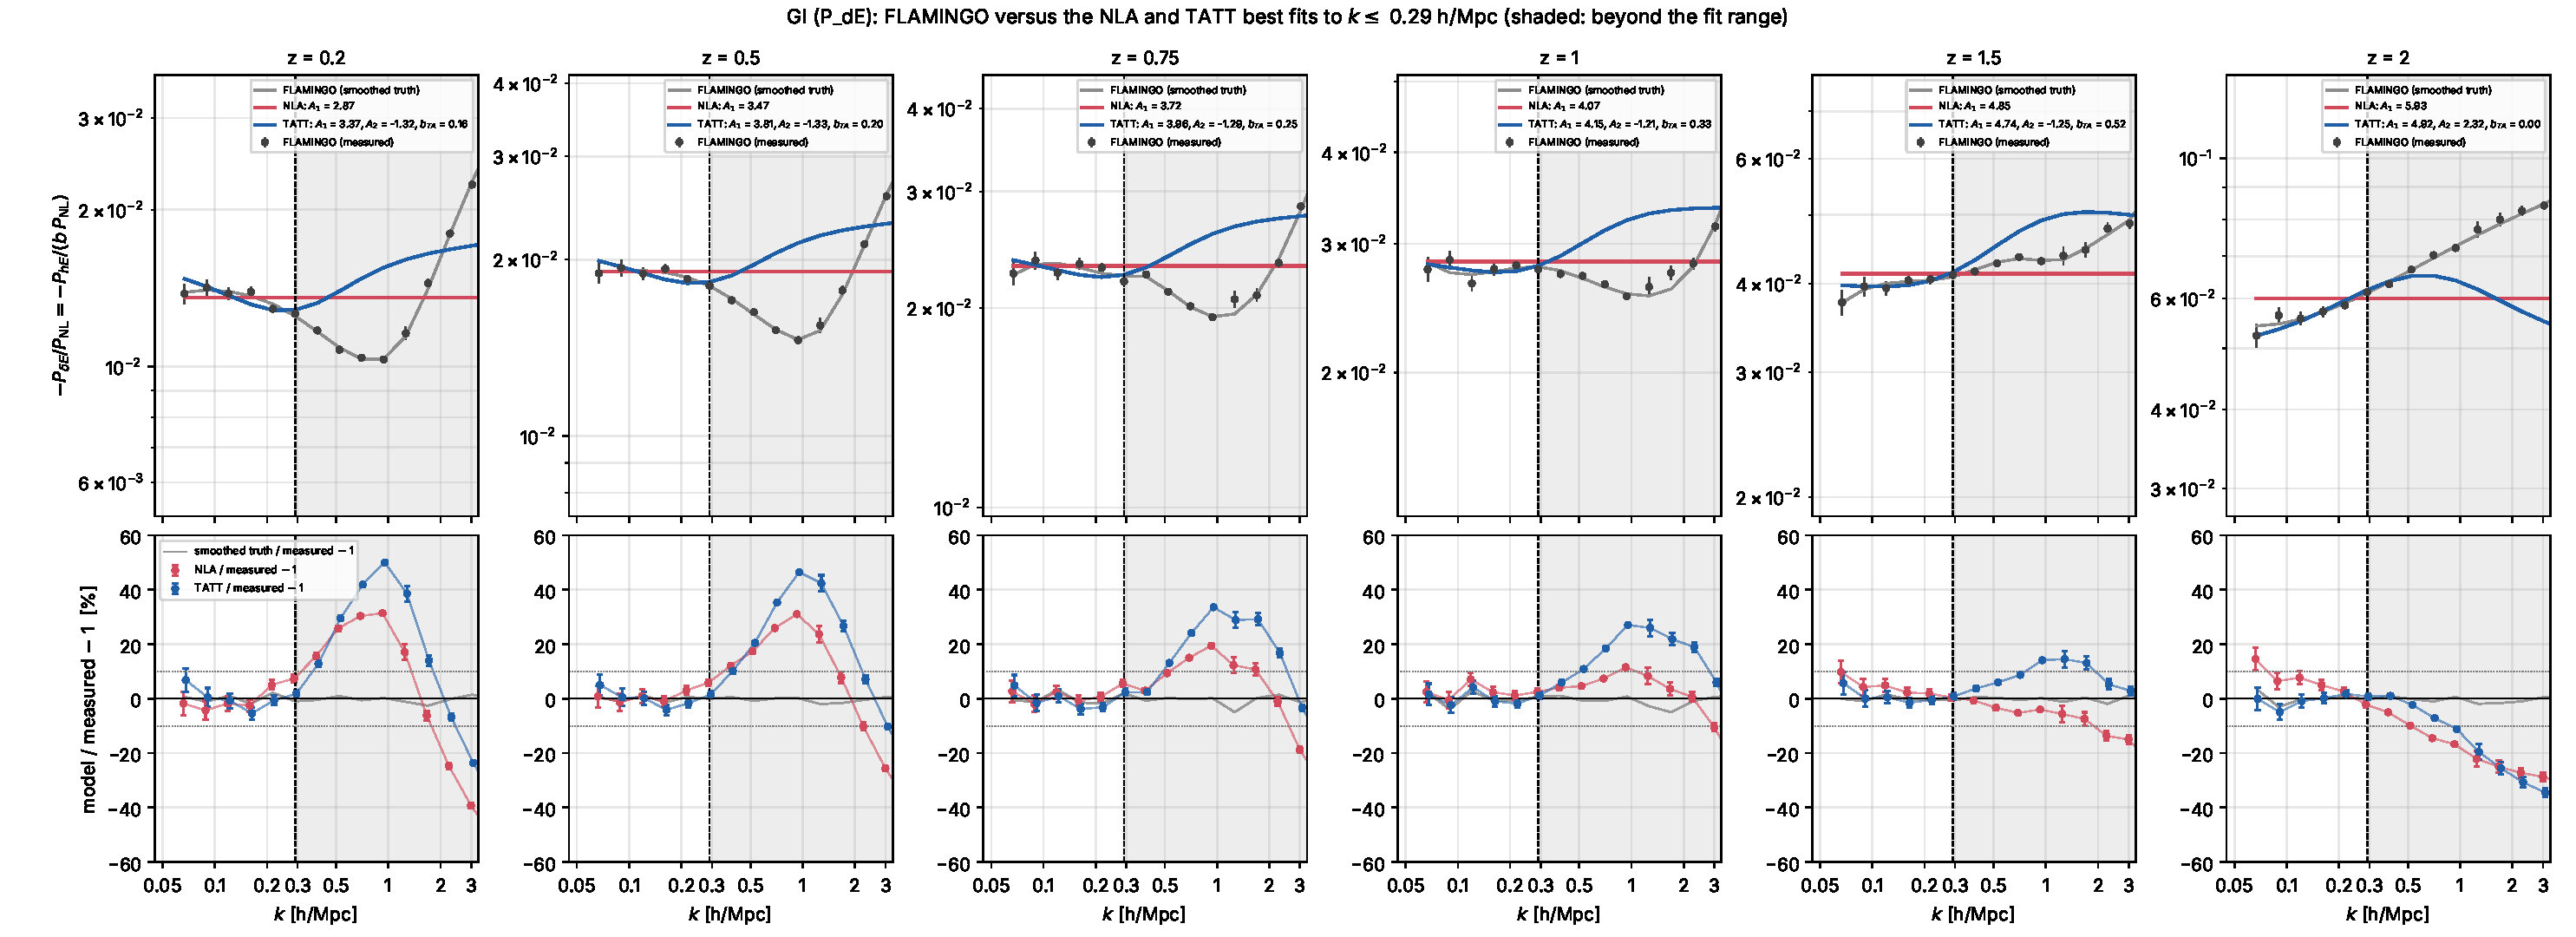
\includegraphics[width=\textwidth]{fig_cmp_GI_k0p29}
\caption{GI, fits to $k \le 0.29\hmpc$ (the TATT GoF cut at most redshifts).}
\label{fig:gi29}
\end{figure}
\begin{figure}[H]\centering
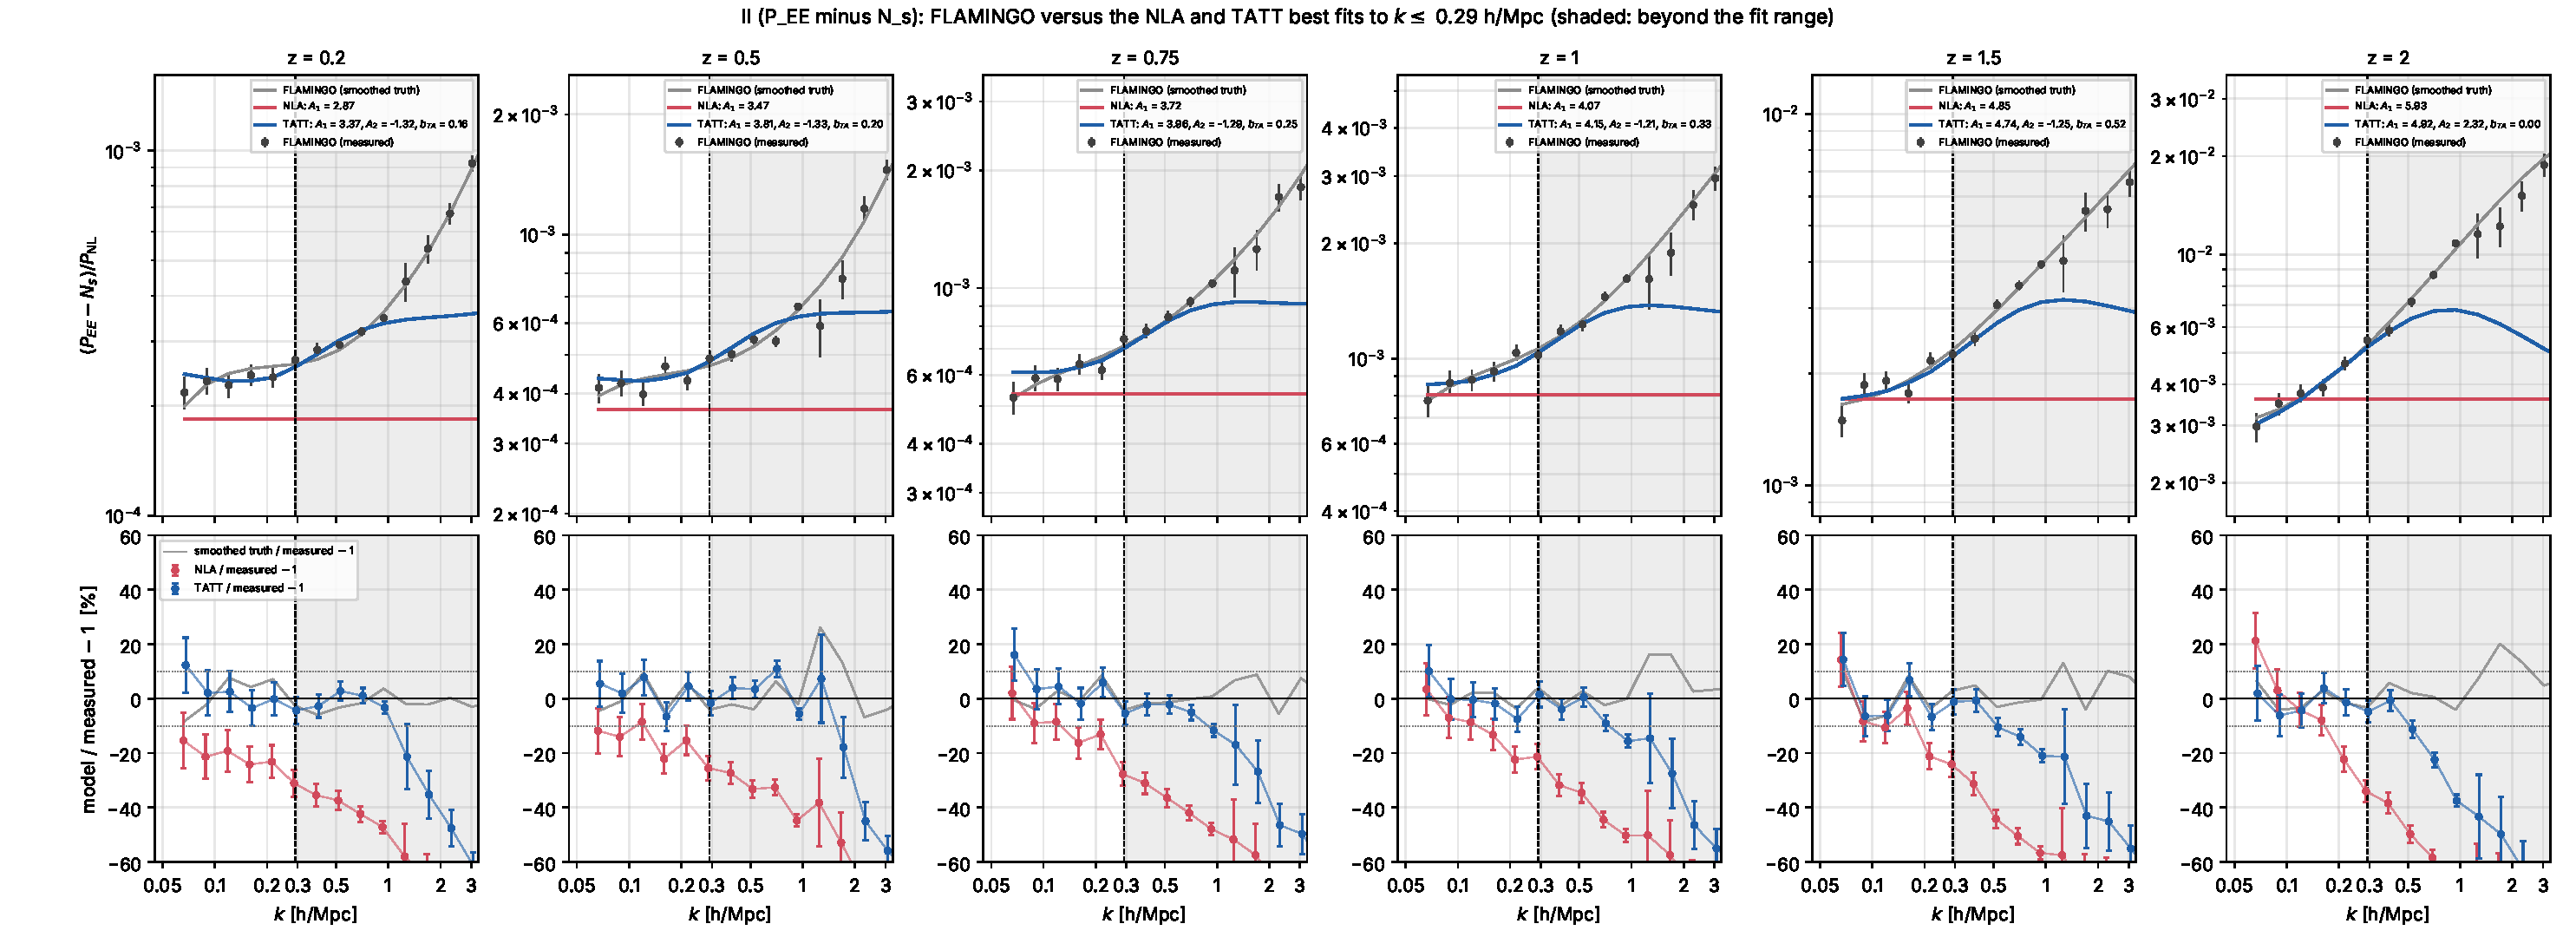
\includegraphics[width=\textwidth]{fig_cmp_II_k0p29}
\caption{II, fits to $k \le 0.29\hmpc$.}
\label{fig:ii29}
\end{figure}
\begin{figure}[H]\centering
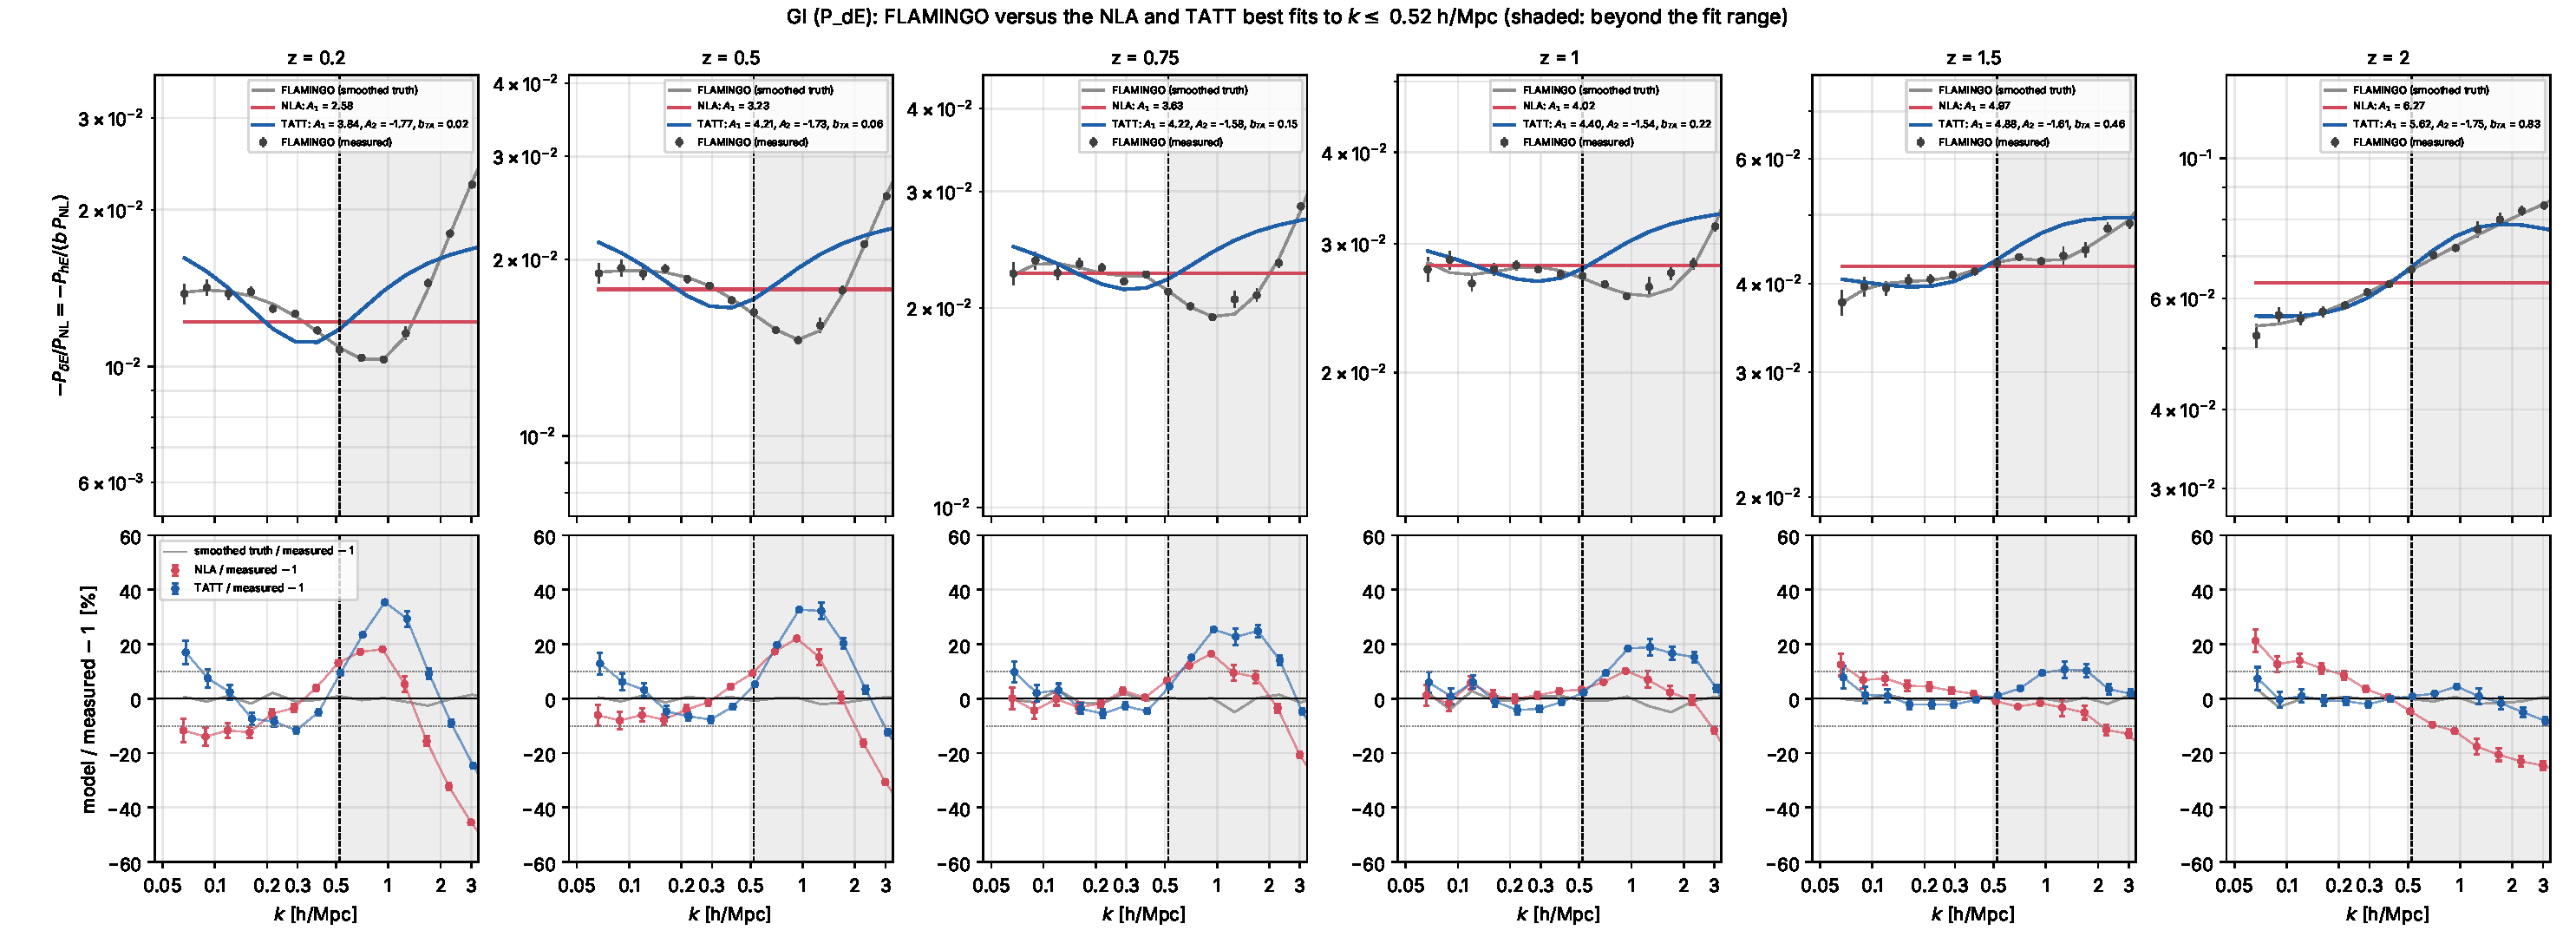
\includegraphics[width=\textwidth]{fig_cmp_GI_k0p52}
\caption{GI, fits to $k \le 0.52\hmpc$ (both models fail; the compromise the
fits make when pushed past the cut).}
\label{fig:gi52}
\end{figure}
\begin{figure}[H]\centering
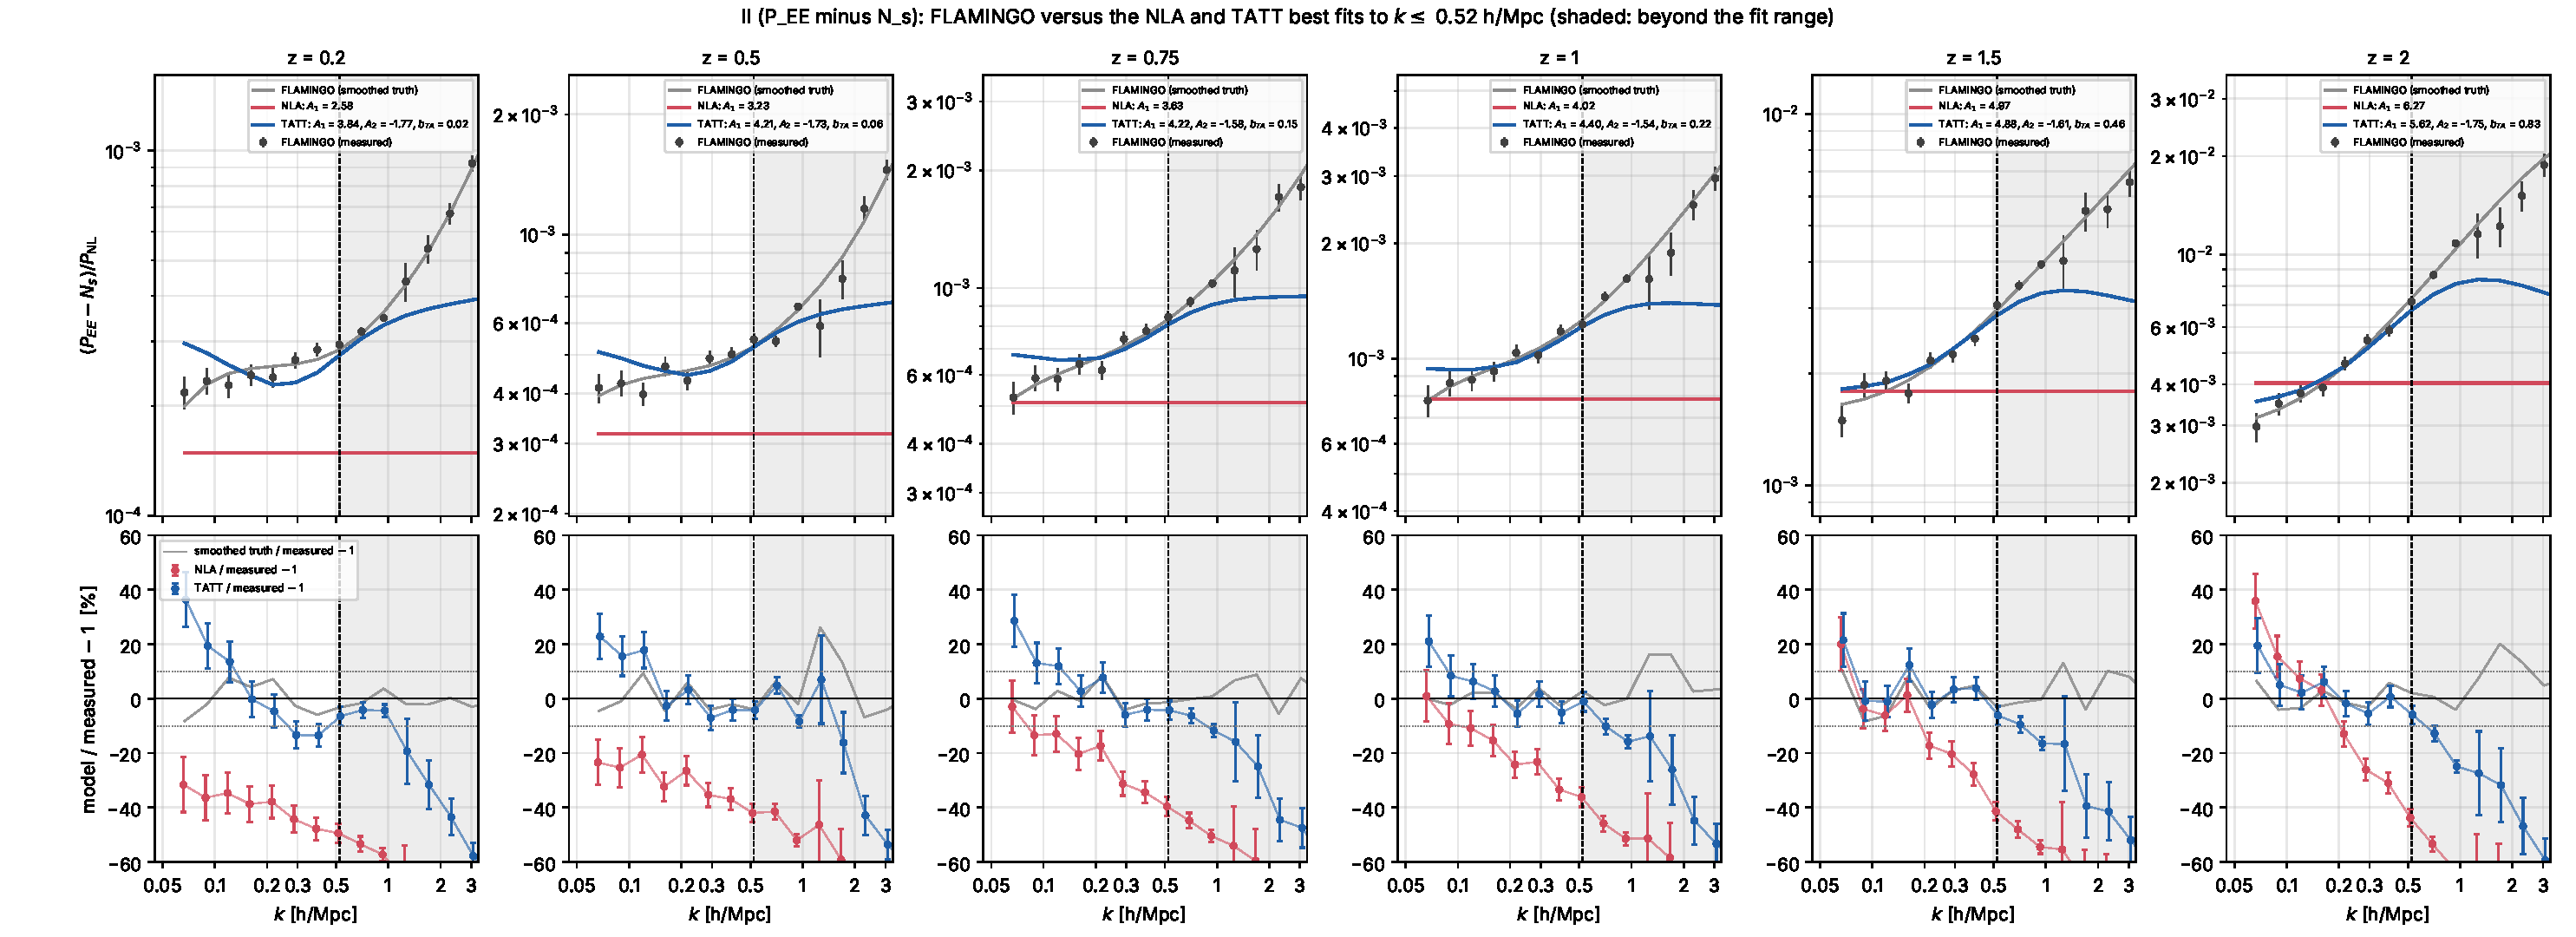
\includegraphics[width=\textwidth]{fig_cmp_II_k0p52}
\caption{II, fits to $k \le 0.52\hmpc$.}
\label{fig:ii52}
\end{figure}
\begin{figure}[H]\centering
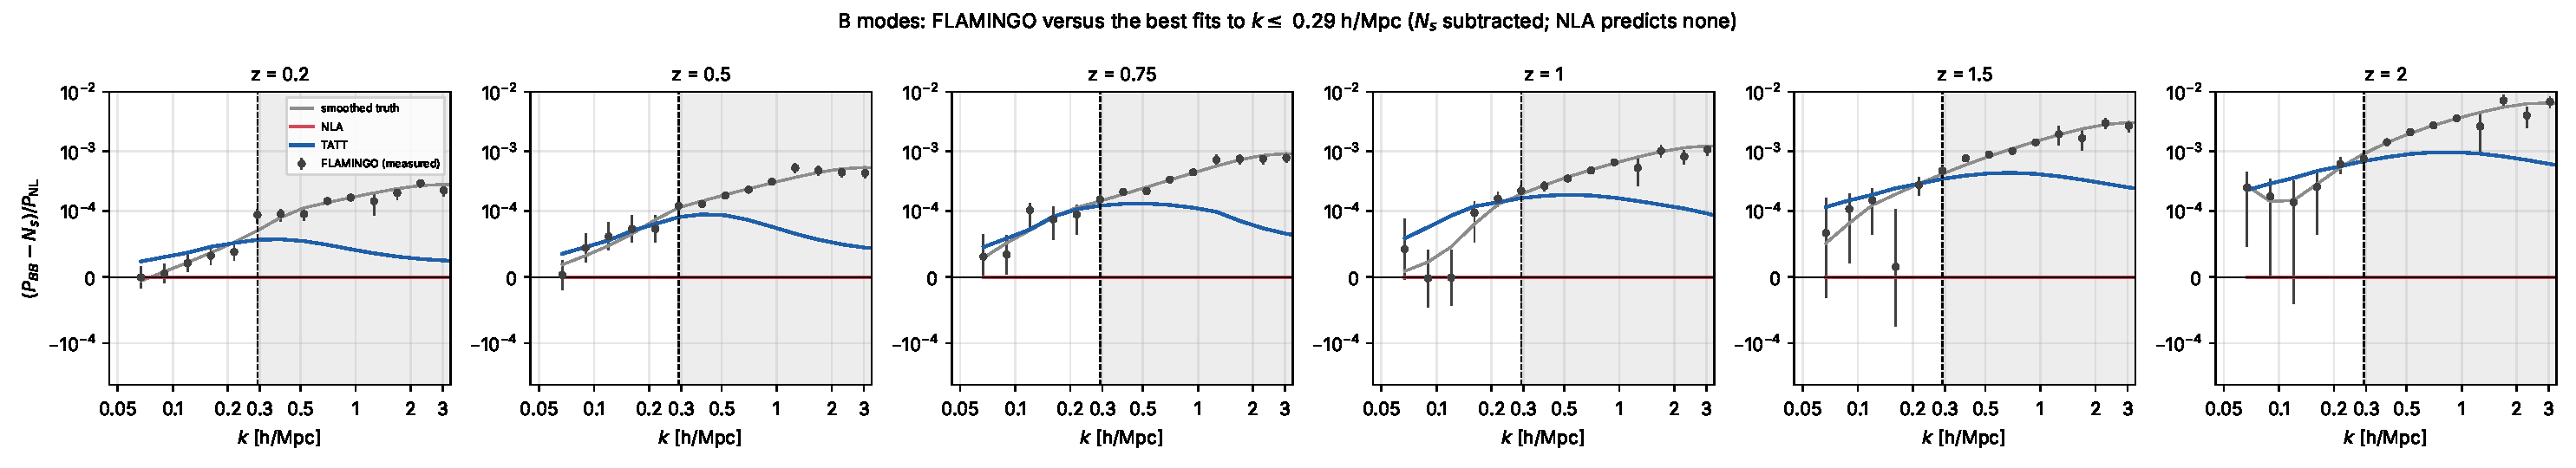
\includegraphics[width=\textwidth]{fig_cmp_BB_k0p29}
\caption{B modes ($P_{BB} - N_s$) against the fits to $k \le 0.29\hmpc$. TATT
predicts a B mode from its quadratic terms; NLA predicts none.}
\label{fig:bb29}
\end{figure}

\section{Goodness of fit as $\chi^2/\nu$}

\paragraph{Definition.} The main summary quotes the goodness of fit as the
$p$-value $p(\kmax) = P[\chi^2_\nu > \chi^2_{\min}(\kmax)]$, with
$\nu(\kmax) = 3N_k(\kmax) - n_{\rm par}$ the number of fitted points minus the
number of free parameters ($n_{\rm par}$ = 1 for NLA, 3 for TATT; $N_k$ the
number of nodes in $0.05 \le k \le \kmax$). The same information as a reduced
chi-square is
\begin{equation}
  \mathrm{GoF}_{\chi^2}(\kmax) \equiv \frac{\chi^2_{\min}(\kmax)}{\nu(\kmax)},
  \qquad
  p < 0.05 \;\Leftrightarrow\; \frac{\chi^2_{\min}}{\nu} > \frac{\chi^2_{0.95}(\nu)}{\nu},
  \label{eq:gofchi2}
\end{equation}
where $\chi^2_{0.95}(\nu)$ is the 95th percentile of the $\chi^2$
distribution with $\nu$ degrees of freedom. The threshold depends on $\nu$:
2.21, 1.94, 1.79, 1.69, 1.62, 1.57, 1.53, 1.47, 1.39 for NLA at $\kmax$ =
0.09, 0.12, 0.16, 0.22, 0.29, 0.39, 0.52, 0.94, 3.04 ($\nu$ = 5 to 41) and
2.60, 2.10, 1.88, 1.75, 1.67, 1.60, 1.56, 1.49, 1.40 for TATT ($\nu$ = 3 to
39). A fixed $\chi^2/\nu$ threshold is therefore not exactly equivalent to a
fixed $p$: it is stricter than $p = 0.05$ at small $\kmax$ (few points) and
looser at large $\kmax$. For the core-combined test ($\nu$ = 9 times larger)
the $p = 0.05$ equivalent is 1.17 to 1.34.

\paragraph{Cut rule in $\chi^2/\nu$ form.} The cut is the last $\kmax$ before
two consecutive grid points with $\chi^2/\nu > \tau$, with $\tau$ either the
$\nu$-dependent value of Eq.~(\ref{eq:gofchi2}) (identical to the $p$ rule)
or a fixed number. Table~\ref{tab:cuts} gives both for $\tau$ = 1.5, 2, 3.

\begin{figure}[H]\centering
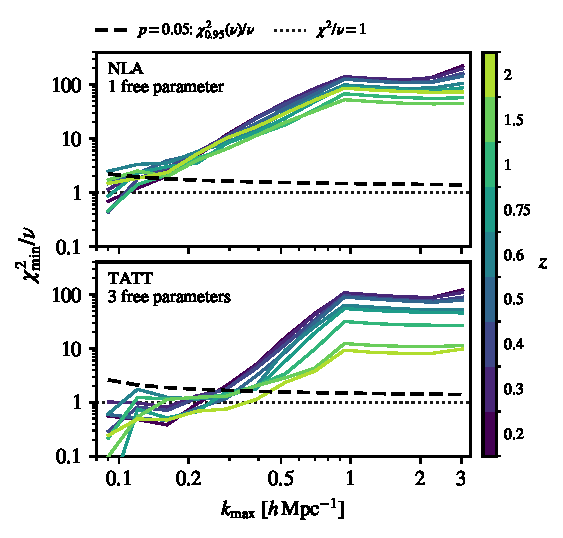
\includegraphics[width=3.5in]{plots/chi2dof/chi2dof}
\caption{$\chi^2_{\min}/\nu$ against $\kmax$ for the nine core snapshots
(refit at every $\kmax$; colour: $z$), NLA (top) and TATT (bottom). Dashed:
the $p = 0.05$ equivalent $\chi^2_{0.95}(\nu)/\nu$; dotted: $\chi^2/\nu = 1$.
Two TATT points at $\kmax = 0.09$ ($\nu = 3$) lie below the panel (0.015 at
$z = 0.75$, 0.099 at $z = 1.5$). The plateau at
$\kmax \ge 1$ is the one-halo regime where the residual grows as fast as the
number of points.}
\label{fig:chi2dof}
\end{figure}
\begin{figure}[H]\centering
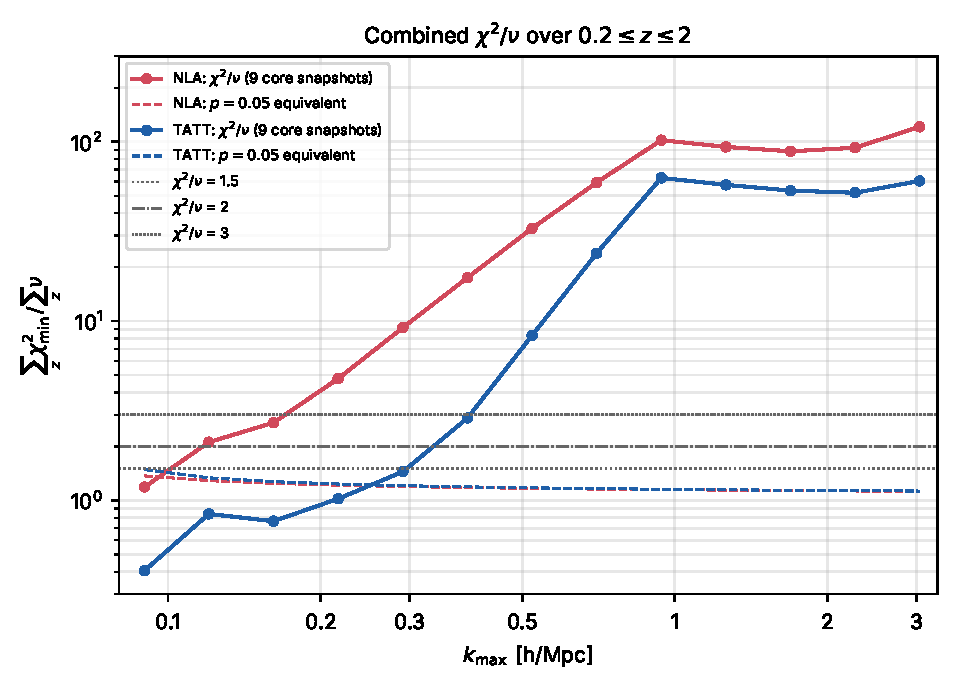
\includegraphics[width=0.6\textwidth]{fig_chi2dof_comb}
\caption{Core-combined $\sum_z \chi^2_{\min} / \sum_z \nu$ with the $p = 0.05$
equivalent for the combined $\nu$ (dashed, model colours).}
\label{fig:chi2comb}
\end{figure}
\begin{figure}[H]\centering
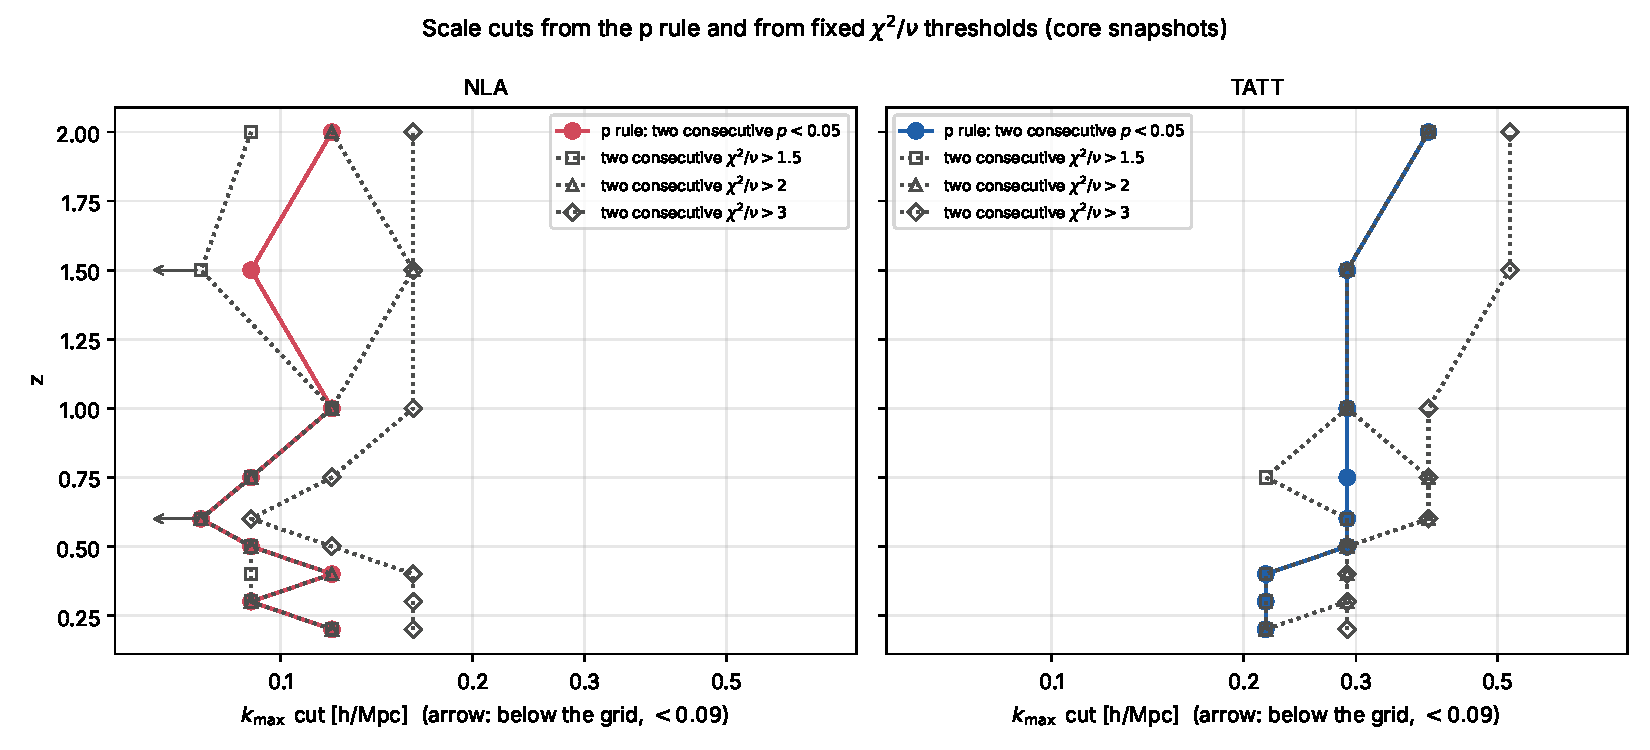
\includegraphics[width=0.9\textwidth]{fig_chi2dof_cuts}
\caption{Scale cuts of the core snapshots from the $p$ rule (filled) and
from fixed $\chi^2/\nu$ thresholds (open). Arrows: the first two grid points
already fail, cut below $0.09\hmpc$.}
\label{fig:chi2cuts}
\end{figure}

\begin{table}[H]\centering\small
\caption{$\chi^2_{\min}/\nu$ per snapshot and $\kmax$ (bold: above the
$p = 0.05$ equivalent threshold, i.e.\ $p < 0.05$; for the combined row the
threshold uses the combined $\nu$). Full grid in \texttt{v3/chi2dof.csv}.}
\label{tab:chi2dof}
\begin{tabular}{llrrrrrr}\toprule
model & $z$ & $k_{\max}=0.12$ & $k_{\max}=0.16$ & $k_{\max}=0.22$ & $k_{\max}=0.29$ & $k_{\max}=0.39$ & $k_{\max}=0.52$\\\midrule
$\nu$ (NLA) &  & 8 & 11 & 14 & 17 & 20 & 23\\
$\nu$ (TATT) &  & 6 & 9 & 12 & 15 & 18 & 21\\
$\chi^2_{0.95}(\nu)/\nu$ (NLA) &  & 1.94 & 1.79 & 1.69 & 1.62 & 1.57 & 1.53\\
$\chi^2_{0.95}(\nu)/\nu$ (TATT) &  & 2.10 & 1.88 & 1.75 & 1.67 & 1.60 & 1.56\\
\midrule
NLA & 0.2 & 1.21 & \textbf{2.02} & \textbf{4.68} & \textbf{11.6} & \textbf{24.4} & \textbf{46.7}\\
NLA & 0.3 & \textbf{2.35} & \textbf{2.63} & \textbf{5.56} & \textbf{10.8} & \textbf{24.0} & \textbf{47.5}\\
NLA & 0.4 & 1.80 & \textbf{2.91} & \textbf{5.09} & \textbf{11.0} & \textbf{23.3} & \textbf{43.6}\\
NLA & 0.5 & \textbf{2.27} & \textbf{3.88} & \textbf{5.11} & \textbf{9.80} & \textbf{18.8} & \textbf{36.2}\\
NLA & 0.6 & \textbf{3.32} & \textbf{3.52} & \textbf{5.67} & \textbf{8.36} & \textbf{14.7} & \textbf{30.8}\\
NLA & 0.75 & \textbf{2.31} & \textbf{3.01} & \textbf{3.48} & \textbf{8.11} & \textbf{13.0} & \textbf{23.9}\\
NLA & 1 & 1.41 & \textbf{2.13} & \textbf{4.32} & \textbf{6.45} & \textbf{11.4} & \textbf{18.0}\\
NLA & 1.5 & \textbf{2.51} & \textbf{1.98} & \textbf{3.92} & \textbf{6.41} & \textbf{11.2} & \textbf{20.1}\\
NLA & 2 & 1.84 & \textbf{2.34} & \textbf{5.15} & \textbf{10.2} & \textbf{16.3} & \textbf{29.5}\\
NLA & all core & \textbf{2.11} & \textbf{2.71} & \textbf{4.78} & \textbf{9.20} & \textbf{17.5} & \textbf{32.9}\\
\midrule
TATT & 0.2 & 0.48 & 0.38 & 0.94 & \textbf{2.03} & \textbf{5.00} & \textbf{16.0}\\
TATT & 0.3 & 0.98 & 0.82 & 1.32 & \textbf{1.74} & \textbf{4.72} & \textbf{14.6}\\
TATT & 0.4 & 0.82 & 0.71 & 1.20 & \textbf{1.78} & \textbf{4.22} & \textbf{11.8}\\
TATT & 0.5 & 0.51 & 0.46 & 0.77 & 1.19 & \textbf{3.07} & \textbf{8.55}\\
TATT & 0.6 & 1.75 & 1.25 & 1.15 & 1.27 & \textbf{1.99} & \textbf{9.36}\\
TATT & 0.75 & 0.75 & 0.51 & 0.67 & 1.57 & \textbf{1.76} & \textbf{5.86}\\
TATT & 1 & 1.24 & 1.15 & 1.20 & 1.38 & \textbf{2.03} & \textbf{3.39}\\
TATT & 1.5 & 0.54 & 1.13 & 1.25 & 1.30 & \textbf{2.01} & \textbf{2.86}\\
TATT & 2 & 0.49 & 0.47 & 0.69 & 0.75 & 1.13 & \textbf{2.35}\\
TATT & all core & 0.84 & 0.77 & 1.02 & \textbf{1.45} & \textbf{2.88} & \textbf{8.32}\\
\bottomrule\end{tabular}
\end{table}

\begin{table}[H]\centering\small
\caption{Cuts (h/Mpc) from the $p$ rule and from fixed $\chi^2/\nu$
thresholds 1.5, 2, 3 (two consecutive failures), and $\chi^2/\nu$ at the
$p$-rule cut and at the next grid point. \texttt{v3/chi2dof\_cuts.csv}.}
\label{tab:cuts}
\resizebox{\textwidth}{!}{\begin{tabular}{l rrrr rrrr rr rr}\toprule
$z$ & \multicolumn{4}{c}{NLA cut} & \multicolumn{4}{c}{TATT cut} & \multicolumn{2}{c}{NLA $\chi^2/\nu$} & \multicolumn{2}{c}{TATT $\chi^2/\nu$}\\
\cmidrule(lr){2-5}\cmidrule(lr){6-9}\cmidrule(lr){10-11}\cmidrule(lr){12-13}
 & $p$ & 1.5 & 2 & 3 & $p$ & 1.5 & 2 & 3 & at cut & next & at cut & next\\\midrule
0.2 & 0.12 & 0.12 & 0.12 & 0.16 & 0.22 & 0.22 & 0.22 & 0.29 & 1.21 & 2.02 & 0.94 & 2.03\\
0.3 & 0.09 & 0.09 & 0.09 & 0.16 & 0.22 & 0.22 & 0.29 & 0.29 & 1.14 & 2.35 & 1.32 & 1.74\\
0.4 & 0.12 & 0.09 & 0.12 & 0.16 & 0.22 & 0.22 & 0.29 & 0.29 & 1.80 & 2.91 & 1.20 & 1.78\\
0.5 & 0.09 & 0.09 & 0.09 & 0.12 & 0.29 & 0.29 & 0.29 & 0.29 & 1.46 & 2.27 & 1.19 & 3.07\\
0.6 & $<0.09$ & $<0.09$ & $<0.09$ & 0.09 & 0.29 & 0.29 & 0.39 & 0.39 & 2.47 & 3.32 & 1.27 & 1.99\\
0.75 & 0.09 & 0.09 & 0.09 & 0.12 & 0.29 & 0.22 & 0.39 & 0.39 & 0.86 & 2.31 & 1.57 & 1.76\\
1 & 0.12 & 0.12 & 0.12 & 0.16 & 0.29 & 0.29 & 0.29 & 0.39 & 1.41 & 2.13 & 1.38 & 2.03\\
1.5 & 0.09 & $<0.09$ & 0.16 & 0.16 & 0.29 & 0.29 & 0.29 & 0.52 & 1.71 & 2.51 & 1.30 & 2.01\\
2 & 0.12 & 0.09 & 0.12 & 0.16 & 0.39 & 0.39 & 0.39 & 0.52 & 1.84 & 2.34 & 1.13 & 2.35\\
\bottomrule\end{tabular}}
\end{table}

\paragraph{Reading.} With $\tau = 2$ the cuts are the $p$-rule cuts except at
$z$ = 0.3, 0.4 (TATT: 0.29 instead of 0.22), $z$ = 0.6, 0.75 (TATT: 0.39
instead of 0.29) and $z = 1.5$ (NLA: 0.16 instead of 0.09), all one grid step
looser; $\tau = 1.5$ is the $p$ rule within one step (four cases one step
tighter); $\tau = 3$ moves the cuts one to two grid steps out (NLA 0.09 to
0.16, TATT 0.29 to 0.52). At the $p$-rule
cut the reduced chi-square is 0.9 to 2.5 (NLA) and 0.9 to 1.6 (TATT); one
step beyond it is 2.0 to 3.3 (NLA) and 1.7 to 3.1 (TATT), and two steps
beyond 2.0 to 5.7 and 2.9 to 9.4 (for $z = 0.6$, NLA, the two columns are
the values at 0.09 and 0.12 since the cut is below the grid). The $\chi^2/\nu$ rises by a factor 2 to 3 per
grid step between 0.2 and 0.9$\hmpc$ for both models, so the cut is not
sensitive to the threshold at the level of one grid step (the grid spacing is
a factor 1.35 in $k$). The core-combined curve (Fig.~\ref{fig:chi2comb})
gives NLA 2.1 at $\kmax = 0.12$ and TATT 1.0 at 0.22, 1.5 at 0.29, 2.9 at
0.39, which is the same ordering as the combined $p$-values of the main
summary ($10^{-7}$ at 0.12 for NLA; $5 \times 10^{-4}$ at 0.29 for TATT).

For the paper the simplest statement is: ``we define the goodness of fit as
$\chi^2_{\min}/\nu$ of the fit to the three FLAMINGO spectra at
$0.05 \le k \le \kmax$ and place the cut at the largest $\kmax$ before
$\chi^2_{\min}/\nu$ exceeds 2 at two consecutive grid points; this coincides
with the $p < 0.05$ criterion to within one grid step.''

\section{Code}
\begin{itemize}\sloppy
\item \texttt{v3/compare\_fits.py} (listed below): rebuilds the model curves
  from the stored best fits (\texttt{v3/v3.npz}, \texttt{NLA\_x},
  \texttt{TATT\_x}) with \texttt{fit\_tatt\_flamingo.TATTModel} on the FLAMINGO
  $P_{\rm NL}$ and $b(k)$ of \texttt{v2/fits.npz}; makes
  \texttt{fig\_cmp\_\{GI,II,BB\}\_k\{0p16,0p29,0p52\}}, \texttt{fig\_chi2dof},
  \texttt{fig\_chi2dof\_comb}, \texttt{fig\_chi2dof\_cuts},
  \texttt{chi2dof.csv}, \texttt{chi2dof\_cuts.csv} (all in \texttt{v3/}).
\item \texttt{v3/v3\_flamingo.py}: the fits themselves (unchanged; the
  $\chi^2$ and $\nu$ arrays are read from its output).
\item The table bodies \texttt{report/tab\_chi2dof.tex} and
  \texttt{tab\_chi2dof\_cuts.tex} are generated from the two CSV files.
\end{itemize}
\lstinputlisting{../v3/compare_fits.py}

\end{document}
